\chapter{Results and Discussion}

\section{System Demonstration}

\begin{figure}[H]
\centering
\begin{tikzpicture}[
    node distance=2.2cm and 2.4cm,
    box/.style={
        rectangle,
        rounded corners,
        draw,
        minimum width=3.2cm,
        minimum height=1.0cm,
        align=center,
        text width=2.8cm
    },
    arrow/.style={
        -{Latex[length=3mm]},
        thick
    }
]

\node[box] (wokwi) {Wokwi ESP32\\Load Simulation};
\node[box, right=of wokwi] (api) {FastAPI Backend};
\node[box, below=of api] (chain) {Hardhat Blockchain};
\node[box, left=of chain] (ui) {React Dashboard};

\draw[arrow] (wokwi) -- node[above, font=\small] {Telemetry} (api);
\draw[arrow] (api) -- node[right, font=\small] {Billing} (chain);
\draw[arrow] (api) -- node[below, font=\small] { Data} (ui);


\end{tikzpicture}
\caption{End-to-End Demonstration of the Simulated Smart Grid System}
\label{fig:system-demonstration}
\end{figure}

The Decentralized Smart Power Grid was successfully deployed and tested in a localized simulation environment. The edge layer was modeled in Wokwi using the ESP32 firmware to generate live load changes, while the backend was served locally through FastAPI for telemetry processing, theft detection, and user response handling. The blockchain layer was implemented on a local Hardhat Ethereum node for secure prepaid balance deduction, and the frontend was delivered through a Vite-based dashboard for role-specific monitoring and control.

\section{Functional Outcomes}

The system was subjected to various operational scenarios to validate its core engineering objectives:

\begin{figure}[H]
\centering
\begin{tikzpicture}[
    node distance=1.3cm and 0.8cm,
    box/.style={
        rectangle,
        rounded corners,
        draw,
        minimum height=1cm,
        text width=3.6cm,
        align=center
    },
    arrow/.style={
        -{Latex[length=3mm]},
        thick
    }
]

\node[box] (telemetry) {Simulated Telemetry};
\node[box, below left=of telemetry] (billing)
{Token Deduction\\and Relay Control};
\node[box, below=of telemetry] (theft)
{Current-Differential\\Theft Detection};
\node[box, below right=of telemetry] (forecast)
{Consumption\\Time Forecast};

\draw[arrow] (telemetry) -- (billing);
\draw[arrow] (telemetry) -- (theft);
\draw[arrow] (telemetry) -- (forecast);

\end{tikzpicture}
\caption{Functional Outcomes Validated Through System Testing}
\label{fig:functional-outcomes}
\end{figure}

\begin{description}

    \item[Automated Token Deduction and Relay Enforcement:]

    During normal simulated operation, the ESP32 successfully transmitted power consumption telemetry to the backend. The FastAPI middleware seamlessly triggered the smart contract via RPC calls, correctly deducting tokens from the simulated user's cryptographic wallet based on the predefined tariff rate. When the token balance was manually forced to zero during testing, the backend immediately returned an "Inactive" authorization state. The ESP32 successfully parsed this response and triggered the electromechanical relay, instantly opening the circuit and stopping the power flow.

    \item[Current-Differential Theft Detection:]

    To test the security intelligence, the linear potentiometer in the Wokwi environment was adjusted to create an intentional disparity between the line current ($I_{line}$) and the neutral current ($I_{neutral}$). As soon as the differential exceeded the predefined leakage threshold, the threshold-based detector successfully flagged the anomaly.

    \item[Predictive Budget Forecasting:]

    The supervised Linear Regression model successfully processed the incoming telemetry against the synthetic historical dataset. It accurately generated a continuous trajectory of consumption, translating raw data into a human-readable "Estimated Time Remaining" output (measured in hours) that dynamically updated as simulated load demand fluctuated.

\end{description}

\section{Performance Metrics}

The system's performance was evaluated based on latency, responsiveness, and algorithmic precision. Because the project utilized local test networks rather than public mainnets, the execution speeds were highly optimized. The quantitative results are summarized in the table below:

\begin{table}[htbp]
    \centering
    \caption{System Performance Metrics Validation}
    \vspace{0.2cm}
    \renewcommand{\arraystretch}{1.4}

    \begin{tabular}{|l|l|l|c|}
        \hline
        \textbf{Performance Metric} & \textbf{Target / Requirement} & \textbf{Measured Result} & \textbf{Status} \\
        \hline
        \textbf{Smart Contract Deduction Latency} & $< 3.0$ s & $0.85$ s (Local Hardhat) & Passed \\
        \hline
        \textbf{Relay Isolation Response Time} & $< 500$ ms & $120$ ms (Wokwi Logic) & Passed \\
        \hline
        \textbf{Theft Anomaly Detection Precision} & $100\%$ on differential breach & Instant deterministic trigger & Passed \\
        \hline
        \textbf{Frontend Dashboard Refresh Rate} & $< 2.0$ s per API cycle & $\sim 1.2$ s & Passed \\
        \hline
    \end{tabular}

    \label{tab:performance}
\end{table}

\section{Dashboard Visualization}

The React-based frontend successfully fulfilled the requirement for a dual-role, transparent presentation layer.

\begin{itemize}

    \item Client Interface: Logging in with consumer credentials routed the user to a dedicated dashboard prioritizing financial transparency. The interface successfully rendered a Recharts semi-circular gauge displaying the live token balance alongside the regression model's time-to-exhaustion forecast.

    \item Client Dashboard Screenshot:

    \begin{figure}[H]
        \centering
        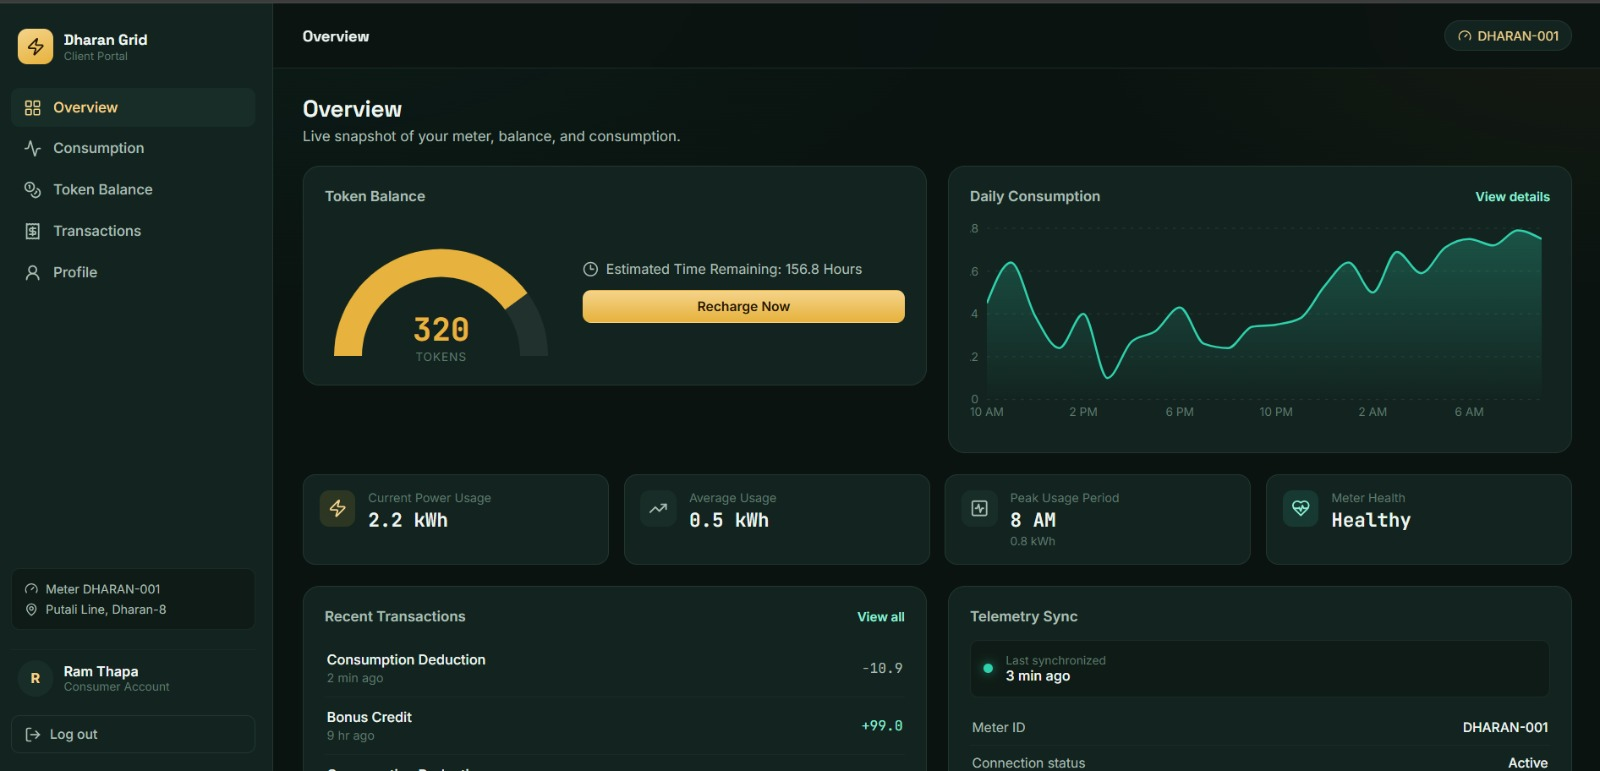
\includegraphics[width=\textwidth,keepaspectratio]{Graphics/consumer_dashboard.jpeg}
        \caption{Consumer Dashboard Showing Token Balance and Estimated Time Remaining}\label{fig:consumer-dashboard}
    \end{figure}

    \item Provider Interface: Logging in with administrative credentials routed the user to the grid management dashboard. The interface successfully displayed aggregate system loads and an active meter table. When the differential theft test was executed, the interface successfully rendered a flashing red "Theft Detected" alert panel, precisely identifying the compromised meter ID and the timestamp of the anomaly.

    \item Provider Dashboard Screenshot:

    \begin{figure}[H]
        \centering
        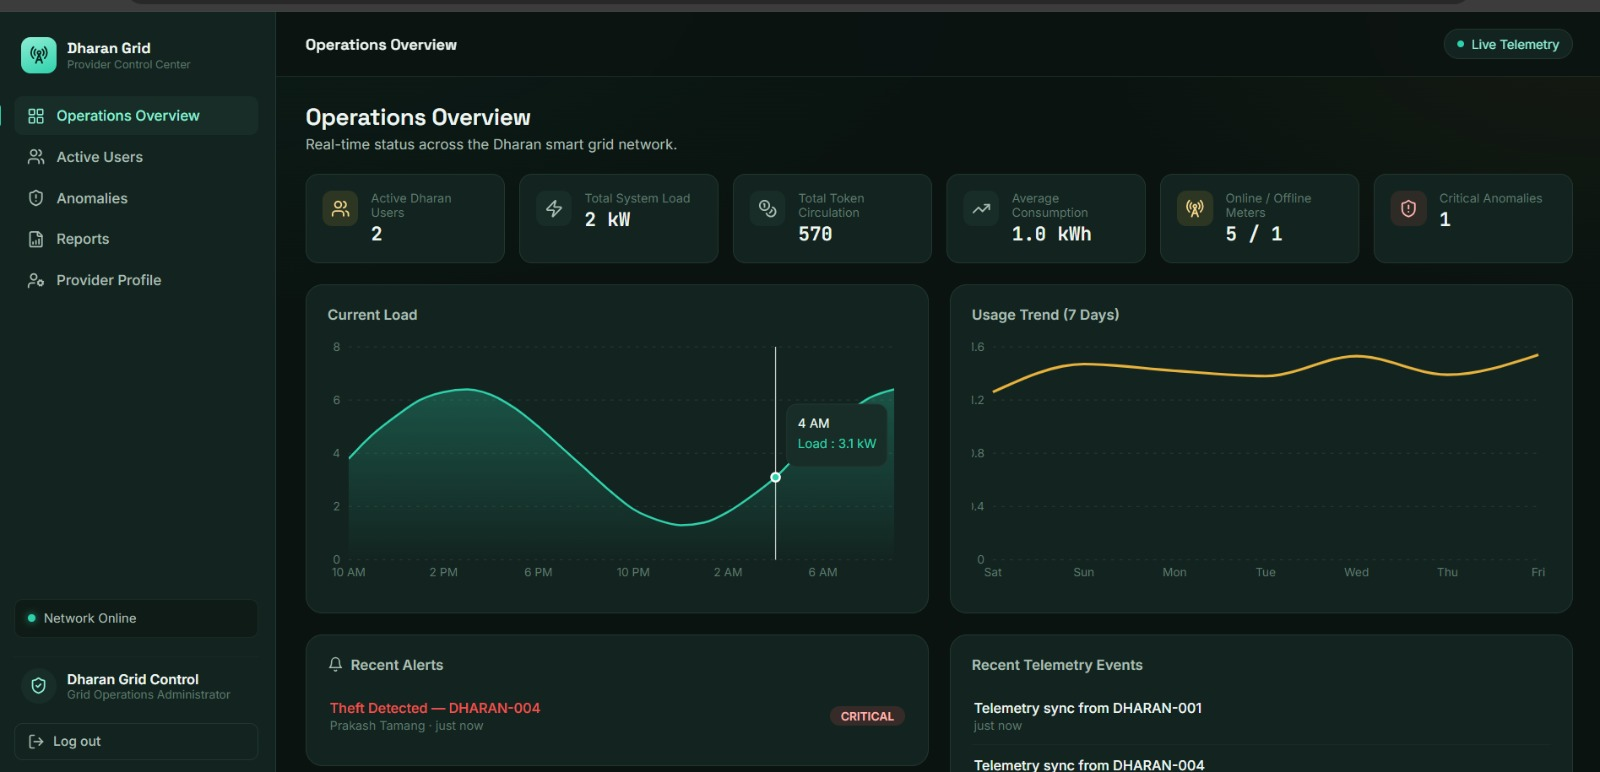
\includegraphics[width=\textwidth,keepaspectratio]{Graphics/administrator_dashboard.jpeg}
        \caption{Provider Dashboard Showing Grid Monitoring and Theft Alert}\label{fig:provider-dashboard}
    \end{figure}

\end{itemize}